% Latex template: mahmoud.s.fahmy@students.kasralainy.edu.eg
% For more details: https://www.sharelatex.com/learn/Beamer

\documentclass[aspectratio=1610]{beamer}					% Document class

\setbeamertemplate{footline}[text line]{%
  \parbox{\linewidth}{\vspace*{-8pt}Probabilistic graphical models\hfill\insertshortauthor\hfill\insertpagenumber}}
\setbeamertemplate{navigation symbols}{}

\usepackage[english]{babel}				% Set language
\usepackage[utf8x]{inputenc}			% Set encoding

\mode<presentation>						% Set options
{
  \usetheme{default}					% Set theme
  \usecolortheme{default} 				% Set colors
  \usefonttheme{default}  				% Set font theme
  \setbeamertemplate{caption}[numbered]	% Set caption to be numbered
}

% Uncomment this to have the outline at the beginning of each section highlighted.
%\AtBeginSection[]
%{
%  \begin{frame}{Outline}
%    \tableofcontents[currentsection]
%  \end{frame}
%}

\usepackage{graphicx}					% For including figures
\usepackage{booktabs}					% For table rules
\usepackage{hyperref}					% For cross-referencing
\usepackage[absolute,overlay]{textpos}
\usepackage{bm}

\title{Probabilistic graphical models}	% Presentation title
\author{Clayton W. Seitz}								% Presentation author
\date{\today}									% Today's date	

\begin{document}

% Title page
% This page includes the informations defined earlier including title, author/s, affiliation/s and the date
\begin{frame}
  \titlepage
\end{frame}

% Outline
% This page includes the outline (Table of content) of the presentation. All sections and subsections will appear in the outline by default.
\begin{frame}{Outline}
  \tableofcontents
\end{frame}

% The following is the most frequently used slide types in beamer
% The slide structure is as follows:
%
%\begin{frame}{<slide-title>}
%	<content>
%\end{frame}


\begin{frame}{Probabilistic graphical models (PGMs)}

\begin{textblock*}{10cm}(1cm,1.5cm)
Say we have a joint probability over gene expression $P(\bm{X})$\\A PGM describes how $P(\bm{X})$ factors\\
\end{textblock*}

\begin{textblock*}{9cm}(1cm,3.5cm)
\textcolor{red}{Markov Random Fields} (MRFs) e.g., Ising model
\begin{equation*}
P(\bm{X};\Theta) = \frac{1}{Z}\prod_{i=1}^{N}P(\bm{X_{i}},\mathcal{C}(X_{i});\Theta_{i})
\end{equation*}
\end{textblock*}

\begin{textblock*}{7cm}(1cm,6.5cm)
\textcolor{red}{Bayesian Network} (BNs) - include causality
\begin{equation*}
P(\bm{X}|\mathcal{G},\Theta) = \prod_{i=1}^{N}P(\bm{X_{i}}|\mathcal{C}(X_{i}),\Theta_{i})
\end{equation*}
\end{textblock*}


\begin{textblock*}{5cm}(10.75cm,1cm)
\begin{figure}
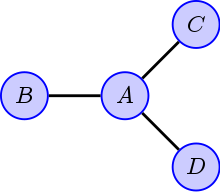
\includegraphics[width=4cm]{mrf.png}
\end{figure}
\end{textblock*}

\begin{textblock*}{5cm}(10.75cm,5cm)
\begin{figure}
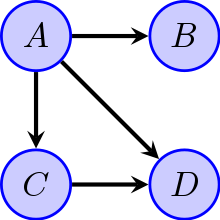
\includegraphics[width=2.75cm]{bayes-net.png}
\end{figure}
\end{textblock*}

\begin{textblock*}{15cm}(1cm,9cm)
BNs as well as hybrid models have been used to examine gene expression
\end{textblock*}

\end{frame}

\begin{frame}{Markov random fields}

\begin{equation*}
P(\mathbf{x}) = \frac{\exp\left(-H(\mathbf{x})\right)}{\sum_{i} \exp\left(-H(\mathbf{x}_{i})\right)}
\end{equation*}

Suppose the energy function can be written as a sum over cliques: 
\begin{equation*}
H(\mathbf{x}) = \sum_{n} \tilde{\psi}_{n}(c_{n})
\end{equation*}
Let $\psi_{n} = \log \tilde{\psi_{n}}$, which means $P(\mathbf{x})$ factors according to 
\begin{equation*}
P(\mathbf{x}) = \frac{\prod_{n} \psi_{n}(c_{n})}{\sum_{i} \prod_{n} \psi_{n}(c_{n})}
\end{equation*}


\end{frame}



\section{References}

% Adding the option 'allowframebreaks' allows the contents of the slide to be expanded in more than one slide.
\begin{frame}[allowframebreaks]{References}
	\tiny\bibliography{references}
	\bibliographystyle{apalike}
\end{frame}

\end{document}